\documentclass[border=6pt]{standalone}
% Shared preamble for web figures.  Each figure is a standalone .tex that
% \input's this file; scripts/make-figures.sh turns it into an SVG.
% Handouts pull the same file with \fig{Unit_X/<name>}.
\usepackage[T1]{fontenc}
\usepackage{helvet}
\renewcommand{\familydefault}{\sfdefault}
\renewcommand{\ttdefault}{pcr}  % Courier: a real Type 1 typewriter font
\usepackage{amsmath}
\usepackage{tikz}
\usetikzlibrary{arrows.meta,positioning,calc,shapes.symbols,shapes.geometric}

% Who makes the rules is the point of most diagrams in this book, so the
% colors mean the same thing everywhere: blue is a person, orange is the
% computer, green is an answer, pink is the human brain.
\definecolor{person}{HTML}{2C6FAE}
\definecolor{machine}{HTML}{D35400}
\definecolor{result}{HTML}{1E8449}
\definecolor{brainpink}{HTML}{C2185B}
\definecolor{ink}{HTML}{2C3E50}

\tikzset{
  doodle/.style={line width=1.5pt, line cap=round, line join=round, draw=ink},
  box/.style={draw, rounded corners=5pt, line width=1.1pt, align=center,
              inner sep=7pt, minimum height=1.0cm, font=\small},
  personbox/.style={box, draw=person, fill=person!10},
  machinebox/.style={box, draw=machine, fill=machine!10},
  resultbox/.style={box, draw=result, fill=result!10},
  plainbox/.style={box, draw=ink!70, fill=ink!4},
  flow/.style={-{Stealth[length=8pt]}, line width=1.4pt, draw=ink},
}

% A person (blue) and a robot head (orange) as small icons.
% \personicon{x}{y}{scale}   \roboticon{x}{y}{scale}
\newcommand{\personicon}[3]{%
  \begin{scope}[shift={(#1,#2)}, scale=#3]
    \fill[person] (0,0.62) circle (0.28);
    \fill[person, rounded corners=6pt] (-0.42,-0.55) rectangle (0.42,0.28);
  \end{scope}}
\newcommand{\roboticon}[3]{%
  \begin{scope}[shift={(#1,#2)}, scale=#3]
    \draw[machine, line width=1.2pt] (0,0.5) -- (0,0.72);
    \fill[machine] (0,0.78) circle (0.08);
    \draw[machine, line width=1.4pt, fill=machine!12, rounded corners=4pt] (-0.5,-0.45) rectangle (0.5,0.5);
    \fill[ink] (-0.2,0.12) circle (0.08);
    \fill[ink] (0.2,0.12) circle (0.08);
    \draw[ink, line width=1pt] (-0.22,-0.22) -- (0.22,-0.22);
  \end{scope}}

\begin{document}
% \blanklabels (set by 2.2_neuron_blank.tex) swaps each label for a number.
\newcommand{\partlabel}[3]{\ifdefined\blanklabels\node[circle, draw=ink, line width=1pt, fill=white, font=\bfseries, inner sep=2pt] at #1 {#2};\else\node[lab] at #1 {#3};\fi}
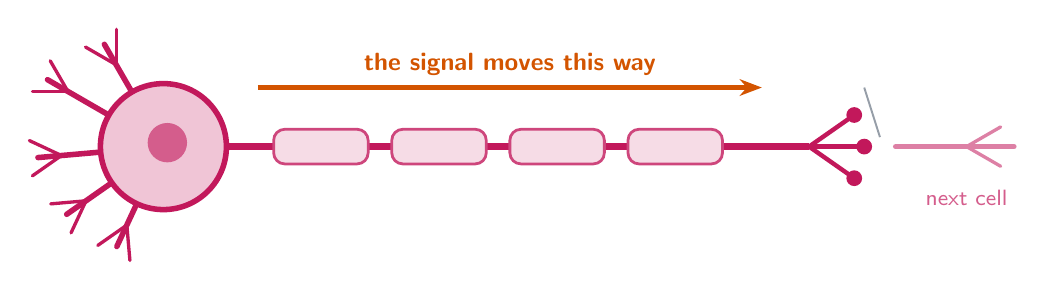
\begin{tikzpicture}[lab/.style={font=\small\bfseries, text=ink, align=center}]
% A neuron: dendrites take signals in, the cell body adds them up, the axon
% carries the signal away, the synapse passes it to the next cell.
\definecolor{cellc}{HTML}{C2185B}
% dendrites
\foreach \a/\l in {120/1.5, 150/1.7, 185/1.6, 215/1.5, 245/1.4} {
  \draw[cellc, line width=2pt, line cap=round] (\a:0.55) -- (\a:\l);
  \draw[cellc, line width=1.2pt, line cap=round] (\a:{\l-0.3}) -- ++(\a+30:0.45);
  \draw[cellc, line width=1.2pt, line cap=round] (\a:{\l-0.3}) -- ++(\a-30:0.45);
}
% cell body
\fill[cellc!25] (0,0) circle (0.8);
\draw[cellc, line width=2pt] (0,0) circle (0.8);
\fill[cellc!70] (0.05,0.05) circle (0.25);
% axon with myelin
\draw[cellc, line width=2.4pt] (0.8,0) -- (8.2,0);
\foreach \x in {1.4, 2.9, 4.4, 5.9} \draw[cellc!80, fill=cellc!15, line width=1pt, rounded corners=4pt] (\x,-0.22) rectangle ++(1.2,0.44);
% terminals
\foreach \a in {-35, 0, 35} {
  \draw[cellc, line width=1.6pt, line cap=round] (8.2,0) -- ++(\a:0.7) coordinate (t\a);
  \fill[cellc] (t\a) circle (0.1);
}
% next cell's dendrite and the synapse gap
\draw[cellc!55, line width=2pt, line cap=round] (9.3,0) -- (10.8,0);
\draw[cellc!55, line width=1.2pt, line cap=round] (10.2,0) -- ++(30:0.5) (10.2,0) -- ++(-30:0.5);
\node[font=\footnotesize, text=cellc!70] at (10.2,-0.65) {next cell};
% signal direction
\draw[flow, draw=machine, line width=1.8pt] (1.2,0.75) -- node[above, font=\small\bfseries, text=machine] {the signal moves this way} (7.6,0.75);
% labels
\partlabel{(-2.6,1.9)}{1}{dendrites\\[-1pt]\footnotesize\mdseries take signals in}
\partlabel{(0.9,-1.45)}{2}{cell body\\[-1pt]\footnotesize\mdseries adds them up}
\partlabel{(4.4,-0.8)}{3}{axon\\[-1pt]\footnotesize\mdseries carries the signal}
\partlabel{(8.9,1.15)}{4}{synapse\\[-1pt]\footnotesize\mdseries a tiny gap}
\draw[ink!50, line width=0.7pt] (8.9,0.75) -- (9.1,0.12);
\end{tikzpicture}
\end{document}
